% !TeX root = ../main.tex

\chapter{系统测试}
本章将会从系统的功能性需求与非功能性需求两个方面,对前两个章节设计与实现的功能进行测试与分析。
功能性需求采用黑盒测试,测试本系统能否正常地提供给用户流水线管理、镜像管理和节点管理的功能,同时也要重点测试人工干预流水线操作后流水线的状态转移。
非功能性测试主要从两个方面进行,首先测试接口在不同并发量下的响应时间,然后从不同作业量下的响应时间和执行时间来测试调度器与执行器处理作业的能力。

\section{测试环境}
系统中需要部署的服务包括Backend服务、调度器服务、执行器服务、数据库服务PostgreSQL、缓存服务Redis、消息队列RocketMQ,镜像服务器,
其中调度器服务与执行器服务为多实例部署。
测试环境硬件配置清单如表\ref{tab:测试环境硬件配置清单}所示。

\begin{table}[ht]
  \centering
  \caption{测试环境硬件配置清单}
  \label{tab:测试环境硬件配置清单}
  \renewcommand{\arraystretch}{1.5}
  \begin{tabular}{|p{1cm}|p{1.5cm}|p{1cm}|p{1cm}|p{1cm}|p{6cm}|}
  \hline
  编号 & 操作系统 & CPU核心数 & 内存(GB)& 硬盘 & 部署服务 \\ \hline
  1 & CentOS & 4 & 8 & 200G & 调度器 \\ \hline
  2 & CentOS & 4 & 8 & 200G & 调度器 \\ \hline
  
  3 & CentOS & 4 & 8 & 200G & 镜像服务器 \\ \hline
  4 & CentOS & 8 & 16 & 200G & 数据库服务PostgreSQL、缓存服务Redis、消息队列RocketMQ \\ \hline
  5 & CentOS & 8 & 16 & 200G & 执行器 \\ \hline
  6 & CentOS & 8 & 16 & 200G & 执行器 \\ \hline
  7 & CentOS & 8 & 16 & 200G & Backend \\ \hline
  \end{tabular}
\end{table}


\section{功能测试}
本小节对系统的三个功能模块中的各个具体用例进行测试,并以测试用例的形式对过程进行了说明。

首先对流水线管理模块进行测试,这一模块的测试点主要在于对流水线的增删改查、配置项配置和人工干预操作,
尤其是触发人工干预操作后,检查状态转移是否符合预期,作业执行过程中的日志和产物是否得到了保存等。

设计作业管理测试用例时,检查点主要有对流水线及其各个子概念的创建、编辑、删除和查看,结果均符合预期,如表\ref{tab:作业管理测试用例表}所示。

\renewcommand{\arraystretch}{1.5}
\begin{longtable}{|p{1.5cm}|p{2.5cm}|p{3cm}|p{3cm}|p{1.5cm}|}
  \caption{作业管理测试用例表} \label{tab:作业管理测试用例表} \\
  \hline
  \multicolumn{1}{|p{1.5cm}|}{测试模块} & \multicolumn{4}{l|}{流水线管理} \\ \hline
  \multicolumn{1}{|p{1.5cm}|}{模块功能} & \multicolumn{4}{l|}{流水线的配置、编辑和查看} \\ \hline
  \multicolumn{1}{|p{1.5cm}|}{测试目的} & \multicolumn{4}{l|}{验证系统是否能正确地对流水线进行配置} \\ \hline
  \endfirsthead
  \multicolumn{5}{c}%
  {{\bfseries \tablename\ \thetable{} -- 续表}} \\
  \hline
  \textbf{用例编号} & \textbf{检查点} & \textbf{操作步骤} & \textbf{预期输出} & \textbf{结果} \\ \hline
  \endhead
  \hline \multicolumn{5}{|r|}{{续下页}} \\ \hline
  \endfoot
  \hline
  \endlastfoot
  用例编号 & 检查点 & 操作步骤 & 预期输出 & 结果 \\ \hline
  1-1-1 & 创建流水线 & 1、进入“我的流水线”Tab页,点击“创建”按钮; \newline 2、录入流水线基本设置; \newline 3、点击“保存”按钮。 & 1、出现创建成功提示信息; \newline 2、在UI界面中看到流水线记录。 & 符合预期 \\ \hline
  1-1-2 & 创建流水线\newline——创建阶段 & 1、在用例1-1-1中切换至拓扑编辑Tab页; \newline 2、在已有的初始阶段上录入基本设置; \newline 3、点击加号增加几个新的阶段并录入基本设置。 & 在流水线的拓扑结构UI界面中看到新创建的阶段 & 符合预期 \\ \hline
  1-1-3 & 创建流水线\newline——创建作业 & 1、在用例1-1-2中点击创建的阶段中的加号; \newline 2、录入基本设置。 & 在流水线的拓扑结构UI界面中看到新创建的作业 & 符合预期 \\ \hline
  1-1-4 & 创建流水线\newline——创建任务 & 1、在用例1-1-3中点击创建的作业中的加号; \newline 2、录入基本设置。 & 在流水线的拓扑结构UI界面中看到新创建的任务 & 符合预期 \\ \hline
  1-2-1 & 编辑流水线 & 1、在“我的流水线”Tab页,在对应流水线处点击“编辑”按钮; \newline 2、修改基本设置; \newline 3、修改拓扑结构。 & 配置页和拓扑结构页的内容更新为编辑后的新内容 & 符合预期 \\ \hline
  1-3-1 & 删除流水线 & 1、在“我的流水线”Tab页,在对应流水线处点击“删除”按钮; \newline 2、在提示弹窗中点击“确认”按钮。 & 出现删除成功提示信息 & 符合预期 \\ \hline
  1-4-1 & 查看流水线配置 & 进入“我的流水线”Tab页,点击“查看”按钮。& 在UI界面中显示了流水线拓扑结构和基本配置 & 符合预期 \\ \hline
\end{longtable}


在对流水线进行适当的增删改查后,系统中成功创建了一条流水线,流水线管理模块功能符合预期,如图\ref{fig:流水线截图}所示,该流水线是对示意图\ref{fig:典型流水线示意图}的实现。
接下来将根据该流水线进行人工干预测试,验证其状态转移是否符合预期。

\begin{figure}[h]
  \centering
  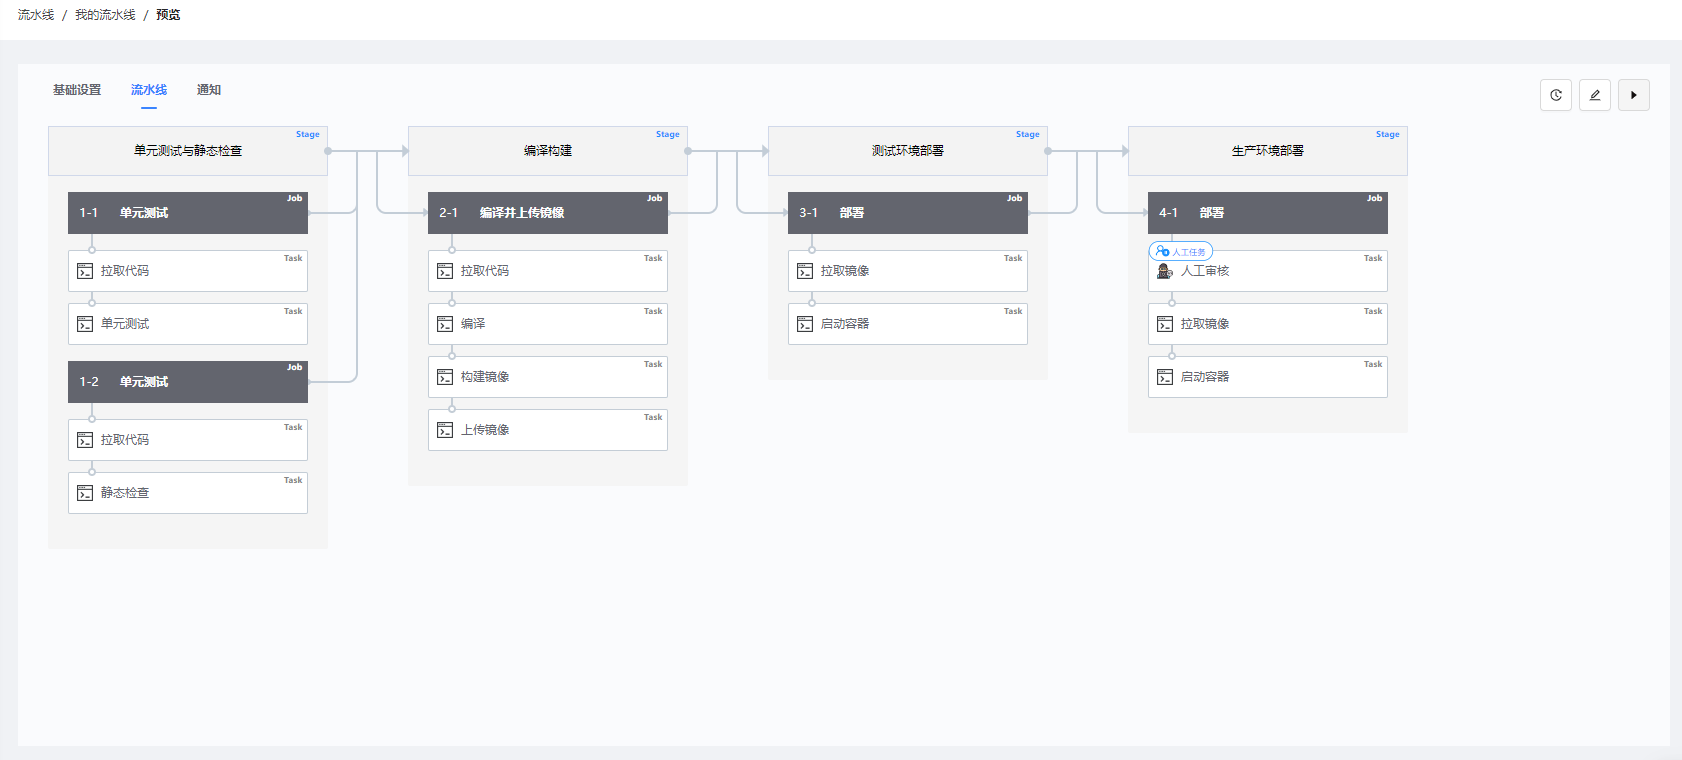
\includegraphics[width=1\textwidth]{流水线截图.png}
  \caption{流水线截图}
  \label{fig:流水线截图}
\end{figure}

对于人工干预流水线,主要的检查点是对流水线及其各个子概念的触发、跳过、重试、取消和人工审核,经过测试,结果均符合预期,如表\ref{tab:人工干预测试用例表}所示。

\renewcommand{\arraystretch}{1.5}
\begin{longtable}{|p{1.5cm}|p{2.5cm}|p{3cm}|p{3cm}|p{1.5cm}|}
  \caption{人工干预测试用例表} \label{tab:人工干预测试用例表} \\
  \hline
  \multicolumn{1}{|p{1.5cm}|}{测试模块} & \multicolumn{4}{l|}{人工干预} \\ \hline
  \multicolumn{1}{|p{1.5cm}|}{模块功能} & \multicolumn{4}{l|}{流水线、阶段、作业的触发、跳过、重试、取消和人工审核} \\ \hline
  \multicolumn{1}{|p{1.5cm}|}{测试目的} & \multicolumn{4}{l|}{验证人工干预后系统的状态流转与作业执行是否符合预期} \\ \hline
  \endfirsthead
  \multicolumn{5}{c}%
  {{\bfseries \tablename\ \thetable{} -- 续表}} \\
  \hline
  \textbf{用例编号} & \textbf{检查点} & \textbf{操作步骤} & \textbf{预期输出} & \textbf{结果} \\ \hline
  \endhead
  \hline \multicolumn{5}{|r|}{{续下页}} \\ \hline
  \endfoot
  \hline
  \endlastfoot
  2-1-1 & 触发流水线 & 1、进入图\ref{fig:流水线截图}所示的流水线预览页面; \newline 2、点击“触发”按钮。& 1、出现触发成功提示信息; \newline 2、在UI界面中看到流水线中作业的运行日志和状态流转。 & 符合预期 \\ \hline
  2-2-1 & 取消流水线 & 在用例2-1-1流水线执行页面中点击“中止”按钮。 & 流水线状态变为已取消,当前正在执行的作业状态变为已取消 & 符合预期 \\ \hline
  2-3-1 & 取消阶段 & 在用例2-1-1中点击正在执行中的阶段上的“中止”按钮。 & 指定的阶段状态变为已取消,阶段内的所有未执行完的作业状态变为已取消 & 符合预期 \\ \hline
  2-4-1 & 重试阶段 & 在用例2-3-1中点击被取消的阶段上的“重试”按钮。 & 原本已被取消的阶段变为执行中,阶段内的作业重新开始运行 & 符合预期 \\ \hline
  2-5-1 & 手动触发作业 & 选择类型为手动触发的作业,点击“触发”按钮 & 在节点资源充足的情况下,手动触发作业由就绪中转为执行中 & 符合预期 \\ \hline
  2-6-1 & 人工审核\newline——审核通过 & 选择类型为人工审核的作业的首个任务,点击“通过”按钮 & 在节点资源充足的情况下,人工审核作业由就绪中转为执行中 & 符合预期 \\ \hline
  2-6-2 & 人工审核\newline——审核驳回 & 选择类型为人工审核的作业的首个任务,点击“驳回”按钮 & 人工审核作业由就绪中转为执行失败 & 符合预期 \\ \hline
  2-7-1 & 取消作业 & 在用例2-1-1执行中的流水线上选择正在执行的流水线点击“取消”按钮 & 作业由执行中转为已取消 & 符合预期 \\ \hline
  2-8-1 & 跳过作业 & 在用例2-1-1执行中的流水线上选择正在执行的流水线点击“跳过”按钮 & 作业由执行中转为已跳过,下一个作业开始执行 & 符合预期 \\ \hline
  2-9-1 & 重试作业 & 在用例2-7-1选择已取消的作业上点击“重试”按钮 & 在节点资源充足的情况下,作业由已取消转为执行中 & 符合预期 \\ \hline
\end{longtable}

接下来对镜像管理模块进行测试用例设计与分析,由于系统中的镜像不仅包含数据库中的记录,也包含镜像服务器中的镜像实体,所以测试对镜像的上传和删除时,需要进入镜像服务器进行验证,同时也要注意测试删除镜像时是否完全清理了Manifest文件和Layer文件。
经过测试,结果均符合预期,如表\ref{tab:人工干预测试用例表}所示。

\renewcommand{\arraystretch}{1.5}
\begin{longtable}{|p{1.5cm}|p{2.5cm}|p{3cm}|p{3cm}|p{1.5cm}|}
  \caption{镜像管理测试用例表} \label{tab:镜像管理测试用例表} \\
  \hline
  \multicolumn{1}{|p{1.5cm}|}{测试模块} & \multicolumn{4}{l|}{镜像管理} \\ \hline
  \multicolumn{1}{|p{1.5cm}|}{模块功能} & \multicolumn{4}{l|}{镜像的制作、删除与上传} \\ \hline
  \multicolumn{1}{|p{1.5cm}|}{测试目的} & \multicolumn{4}{l|}{验证系统对镜像的操作能否正常执行,镜像服务器中镜像是否正常存储与清理} \\ \hline
  \endfirsthead
  \multicolumn{5}{c}%
  {{\bfseries \tablename\ \thetable{} -- 续表}} \\
  \hline
  \textbf{用例编号} & \textbf{检查点} & \textbf{操作步骤} & \textbf{预期输出} & \textbf{结果} \\ \hline
  \endhead
  \hline \multicolumn{5}{|r|}{{续下页}} \\ \hline
  \endfoot
  \hline
  \endlastfoot
  用例编号 & 检查点 & 操作步骤 & 预期输出 & 结果 \\ \hline
  3-1-1 & 制作镜像\newline——dockfile方法 & 1、进入“镜像管理”Tab页,点击“镜像制作”;\newline 2、填写镜像基本信息;\newline 3、上传Dockerfile文件后点击“构建”。& 1、出现制作成功提示信息; \newline 2、在“镜像列表”中查看到新制作的镜像。 & 符合预期 \\ \hline
  3-1-2 & 制作镜像\newline——commit方法 & 1、进入“镜像管理”Tab页,点击“镜像制作”;\newline 2、填写镜像基本信息;\newline 3、选择基础镜像点击“构建”;\newline 4、在终端进行配置操作;5、点击“构建”按钮。 & 1、出现制作成功提示信息; \newline 2、在“镜像列表”中查看到新制作的镜像。 & 符合预期 \\ \hline
  3-2-1 & 编辑镜像 & 1、在用例3-1-1或3-1-2的基础上,点击制作好的镜像上的“编辑”;\newline 2、编辑镜像基本信息后点击“保存”;& 镜像信息更新为编辑后的新内容。 & 符合预期 \\ \hline
  3-3-1 & 上传镜像 & 在用例3-1-1或3-1-2的基础上,点击制作好的镜像上的“上传”。& 1、出现上传成功提示信息;2、在镜像服务器中可以查看到对应镜像。 & 符合预期 \\ \hline
  3-4-1 & 删除镜像 & 在用例3-3-1基础上,点击已上传的镜像点击“删除” & 1、出现删除成功提示信息;2、在镜像服务器上查看对应的Manifest文件和Layer文件已被删除。 & 符合预期 \\ \hline
\end{longtable}

最后对镜像管理模块进行测试用例设计与分析,注意节点的部署和删除等操作会在对应的服务器中安装、启动和卸载服务,测试时需要对服务的可用性进行验证。
节点的Tag与作业的匹配也是节点正常运作的重要测试点,节点部署后需要验证与当前节点Tag相同的作业在此节点上运行。

\renewcommand{\arraystretch}{1.5}
\begin{longtable}{|p{1.5cm}|p{2.5cm}|p{3cm}|p{3cm}|p{1.5cm}|}
  \caption{节点管理测试用例表} \label{tab:节点管理测试用例表} \\
  \hline
  \multicolumn{1}{|p{1.5cm}|}{测试模块} & \multicolumn{4}{l|}{节点管理} \\ \hline
  \multicolumn{1}{|p{1.5cm}|}{模块功能} & \multicolumn{4}{l|}{节点的注册、编辑、部署、上下线与删除} \\ \hline
  \multicolumn{1}{|p{1.5cm}|}{测试目的} & \multicolumn{4}{l|}{验证对系统对节点的操作能否正常执行,与节点服务器的连接与操作是否符合预期} \\ \hline
  \endfirsthead
  \multicolumn{5}{c}%
  {{\bfseries \tablename\ \thetable{} -- 续表}} \\
  \hline
  \textbf{用例编号} & \textbf{检查点} & \textbf{操作步骤} & \textbf{预期输出} & \textbf{结果} \\ \hline
  \endhead
  \hline \multicolumn{5}{|r|}{{续下页}} \\ \hline
  \endfoot
  \hline
  \endlastfoot
  用例编号 & 检查点 & 操作步骤 & 预期输出 & 结果 \\ \hline
  4-1-1 & 注册节点 & 1、进入“节点管理”Tab页,点击“注册新节点”;\newline 2、录入节点基本信息;\newline 3、点击“保存”。& 1、出现注册成功提示信息; \newline 2、在“节点列表”中查看到新注册的节点;\newline 3、查看到节点的状态为“待部署”。 & 符合预期 \\ \hline
  4-2-1 & 编辑节点 & 1、选择用例4-1-1创建的节点,点击“编辑”;\newline 2、编辑节点基本信息;\newline 3、点击“保存”;& 节点信息更新为编辑后的新内容。& 符合预期 \\ \hline
  4-3-1 & 一键部署 & 选择用例4-1-1创建的节点,点击“一键部署”;& 等待五秒左右,节点转变为“已部署”状态;& 符合预期 \\ \hline
  4-4-1 & 节点上线 & 选择用例4-3-1已部署的节点,点击“上线”;& 1、节点转变为“在线”状态;\newline 2、查看到与当前节点Tag相同的作业在此节点上运行。 & 符合预期 \\ \hline
  4-5-1 & 节点下线 & 选择用例4-4-1已上线的节点,点击“下线”;& 节点转变为“离线”状态 & 符合预期 \\ \hline
  4-6-1 & 节点删除 & 1、选择用例4-5-1已下线的节点,点击“删除”;\newline 2、在弹窗中点击“确认” & 出现删除成功提示信息。& 符合预期 \\ \hline
\end{longtable}

\section{性能测试}
接下来将分别测试Backend部分、调度器与执行器的性能。

对于Backend部分,由于用户从前端通过Backend与系统进行数据交互,所以接口的响应时间直接影响用户的实际体验,决定了系统的可用性,故将作为重要的衡量指标。
接下来将使用测试软件 Jmeter 模拟用户请求,对于系统中的所有接口按照不同并发量进行压力测试,并记录平均相应时长。
接口测试情况如表\ref{tab:流水线管理接口响应时间测试表}所示。

\begin{table}[h]
  \centering
  \caption{流水线管理接口响应时间测试表}
  \label{tab:流水线管理接口响应时间测试表}
  \begin{tabular}{clll}
    \toprule
    并发量         & 最大时长            & 平均时长     & 是否符合预期                       \\
    \midrule
    50次         & 310ms              & 158ms     & 符合预期                 \\
    100次        & 408ms              & 180ms     & 符合预期                 \\
    500次        & 580ms              & 255ms     & 符合预期                     \\
    1000次       & 709ms              & 332ms     & 符合预期                     \\
    \bottomrule
  \end{tabular}
\end{table}

可见,在不高于1000次请求的并发量下,系统的平均响应时长均小于1秒,能够满足期望性能,保证系统可用性。

对于CI/CD流水线系统,对作业的处理能力也至关重要,尤其是企业内部往往存在周期性的发布高峰期,任务量会比平时高出数倍,
同时,随着企业服务的用户数量增长和业务扩展,流水线与流水线作业只会越来越多。
因此需要对系统在大作业量下的调度器和执行器性能进行测试,以保证系统能否很好地应对突发流量,并且能够在紧急情况下快速扩容,同时了解系统性能瓶颈,以便日后改进。

对调度器和执行器的整体性能测试计划如表\ref{tab:调度器与执行器性能测试计划表}所示。

\begin{table}[ht]
  \centering
  \caption{调度器与执行器性能测试计划表}
  \label{tab:调度器与执行器性能测试计划表}
  \renewcommand{\arraystretch}{1.5}
  \begin{tabular}{|p{3cm}|p{10cm}|}
  \hline
  测试模块 & 调度器与执行器 \\ \hline
  测试目的 & 测试调度器与执行器在不同作业量下的整体性能 \\ \hline
  测试流水线的结构 & 由4个阶段共五个作业组成,即图\ref{fig:流水线截图}所示结构。\\ \hline
  压测的作业量 & 从10个作业每分钟开始,每次增加5个,直至系统出现明显性能瓶颈为止。\\ \hline
  每次压测时长 & 3分钟\\ \hline
  数据记录 & 任务量、平均响应时长、最长响应时长、任务平均执行耗时、任务最长执行耗时\\ \hline
  \end{tabular}
\end{table}

经过测试,流水线作业数量与响应时长关系如图\ref{fig:作业量与响应时长关系图}所示。
通常来说,企业内每小时平均任务量通常不会超过1000个,约每分钟16个,高峰期每小时平均任务量不会超过2000个,约每分钟33个。
系统要求无论在何种情况下都能在2秒内给予响应,根据测试结果可以发现,在每分钟16个作业的正常情况下,系统的平均响应时长不超过150ms,
在每分钟40个作业的极端情况下,响应时长也刚刚超过1秒,所以调度器和执行器在运行流水线的响应时间上能够满足要求。
调度器和执行器在响应时间上性能优异,这主要是因为调度器主要是进行业务逻辑处理,当需要触发作业时,只需要将作业放入消息队列后异步返回结果即可。

\begin{figure}[h]
  \centering
  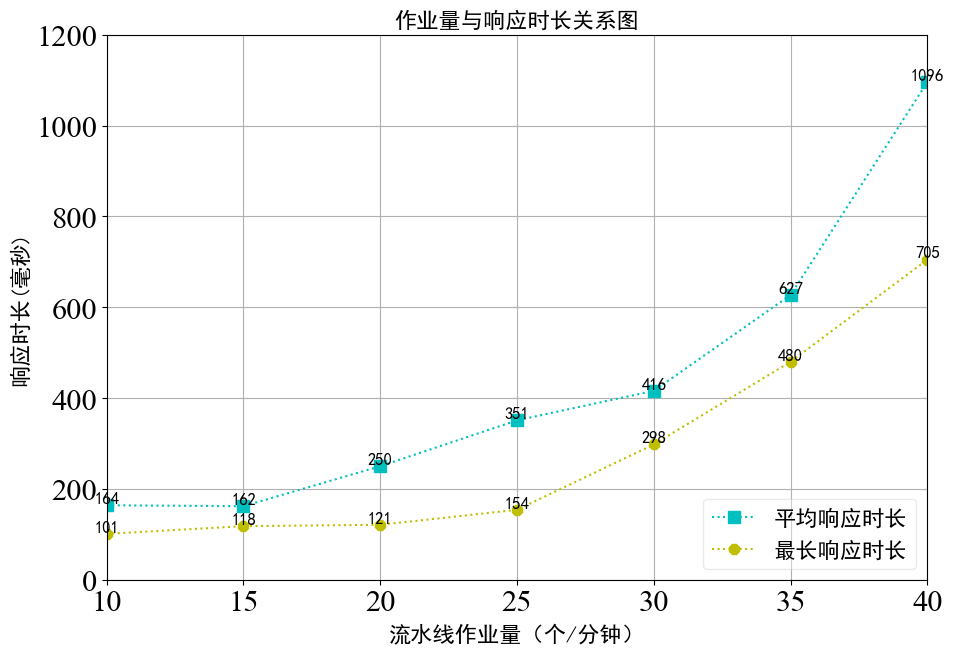
\includegraphics[width=0.8\textwidth]{作业量与响应时间关系图.png}
  \caption{作业量与响应时长关系图}
  \label{fig:作业量与响应时长关系图}
\end{figure}

对于作业执行耗时方面,作业数量与执行时长关系如图\ref{fig:作业量与执行时长关系图}所示。
可以看到,在每分钟作业量小于20个时,测试流水线的平均运行时长均在8分钟左右,可以合理判断当此时调度器与执行器的负载都不高。
同时注意到消息队列中没有出现作业堆积,也说明了当前作业量并没有超出执行器的负载。
当每分钟作业量大于25个时,流水线的最长执行时长陡增,同时查看消息队列发现开始产生作业堆积。
当每分钟作业量大于35个时,流水线的平均执行时长已经超过20分钟,查看消息队列发现产生大量作业堆积,此时系统可用性已经大大降低,
由于调度器是处理完作业才放入消息队列,可见此时调度器的负载较小,主要负载在于执行器。

\begin{figure}[h]
  \centering
  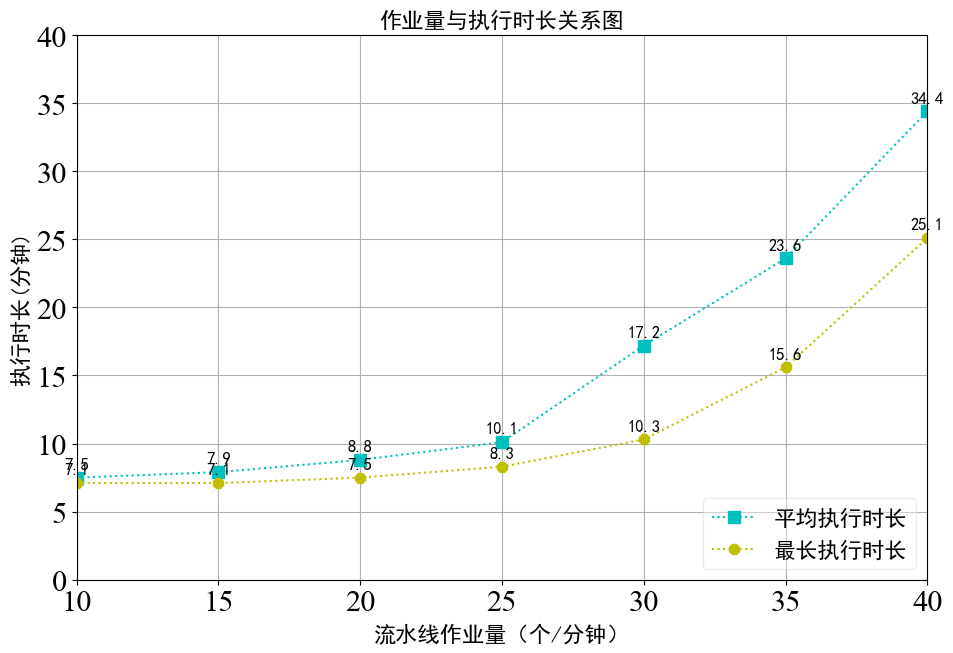
\includegraphics[width=0.8\textwidth]{作业量与执行时长关系图.png}
  \caption{作业量与执行时长关系图}
  \label{fig:作业量与执行时长关系图}
\end{figure}

\section{测试结论}

根据以上测试,在功能方面,本系统在所有的测试用例中的测试结果均符合预期。性能方面,Backend部分接口性能优异,在不高于1000次请求的并发量下,系统的平均响应时长均小于1秒;
调度器和执行器的响应时长在正常情况下不超过150ms,在系统使用高峰期不超过1秒,能够满足用户需求,
对于作业执行时长来说,当每分钟作业量超过35个时,调度器和执行器出现了明显的性能瓶颈,根据分析,该性能瓶颈在于执行器而不在调度器,在后续扩展系统服务能力时应重点考虑扩展执行器集群机器数量或增强硬件配置。
同时由于系统本身能够借助Kubernetes进行横向扩展,现阶段的机器配置能够满足日常需求。



